The overall objective is the implementation of a system based on a reinforcement- or imitation learning algorithm that is able to predict end-to-end vessel trajectories based on historical AIS data. In future steps outside the scope of this thesis, the constructed model could potentially be part of an application used at an marine surveillance center in order to push alerts e.g. in case of an upcoming close encounter between two ships if no party changes its current driving behavior. Before building a suitable system, we defined certain requirements that must be met. Those are:
\paragraph{No dedicated simulation.} Works like the one from \cite{westerlund2021learning} heavily depend on a sophisticated ship simulation to translate actual ship maneuvering like the adjustment of the current speed or rudder angle to realistic ship movements. Although open-source projects such as the \textit{Open Simulation Platform} \cite[]{smogeli2020open} are emerging, a dedicated simulation has to have the ability to reverse historical AIS data to ship controls for thousands of different vessel models because we want the system to act as closely to the normal behavior of a captain approaching or leaving the Bremerhaven port. Therefore, the proposed system must be able to exclusively learn from AIS data with no explicit knowledge of the ship controls.

\paragraph{Complete end-to-end trajectories.}
Methods for predicting sequences like recurrent neuronal networks are only able to output a fixed-sized forecast window based on a fixed-sized input frame. We want the system to be flexible so it can predict complete end-to-end trajectories without the need for previous sequence. Hence, the proposed system must be able to generate full paths purely based on a single input state.

\paragraph{Real-time predictions.} The predefined system observation area as displayed in Fig. \ref{systemObservation} covers approx. $300 km^2$ and thus can potentially perceive more than 50 vessels at a time. A constructed system has to have low computational cost in an effort to operate in near real-time while frequently predicting all future trajectories.


\paragraph{Extensible feature space.}
As previously described, ship maneuvering also depends on non-kinematic factors like weather conditions, tides or surrounding ships. Despite the fact that a first version does not have to incorporate those factors, it should in theory possible to extend the system in straight forward way.


For a better understanding of what an actual application could look like, we illustrate Fig. \ref{fig:systemObservation}.
\begin{figure}[H]
    \centering
    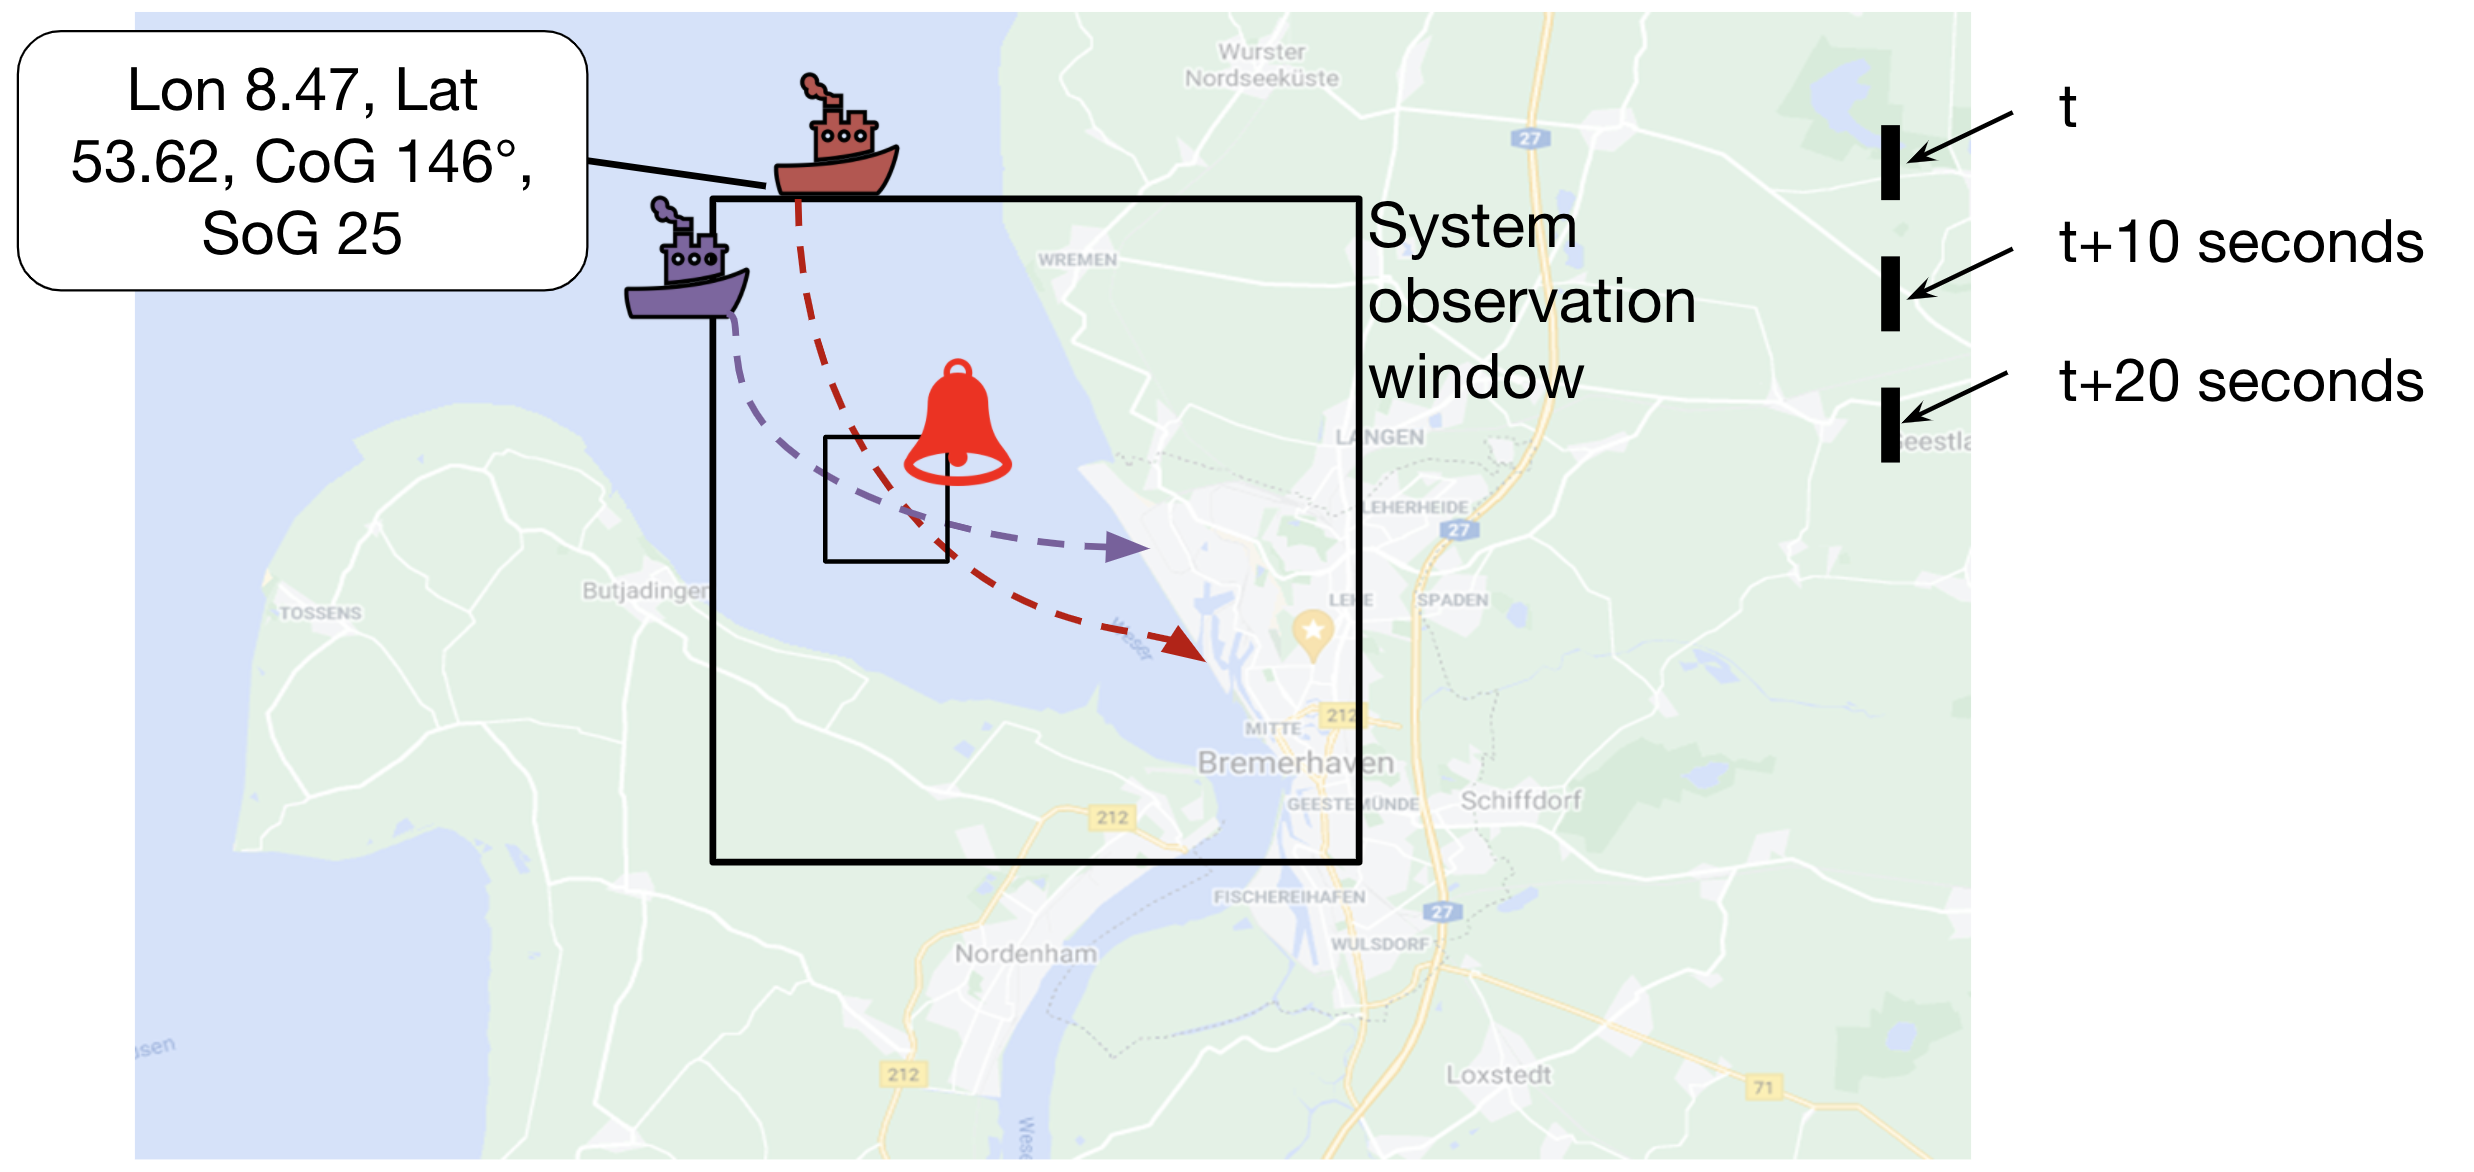
\includegraphics[width=\textwidth]{images/system_observation.png}
    \caption{System observation window}
    \label{fig:systemObservation}
\end{figure}

The system defines a system observation windows for the port and shore of Bremerhaven. As soon as a ship enters this area, the current state with information like position, course over ground (CoG) and speed over ground (SoG) is used to generate a prediction of the path a "normal behaving" instance of this ship would take. Besides drawing the raw path, the system also includes a time component indicated by the dashed line, making it possible to retrace at which specific location the ship will end up after a certain time span. Now, if another ship enters the observation area as well, both path prediction in time will be used to detect possible collisions or close encounters to then yield a warning to the human being in charge of the marine surveillance. It is then up to the expert to contact the captains or wait for upcoming predictions to see if this incidence settles itself.
\par
Apart from the design and implementation of the path prediction system, one intermediate goal is to get a big overview of related work in terms of the anomaly detection of vessels and the recent application of reinforcement learning, most importantly the ones regarding path planning and autonomous control. Diving deep into the field of deep reinforcement learning and imitation learning, we will also have a closer look at the internal mechanism of an actor-critic method. To improve our knowledge of state representation, feature engineering and reward function, we also set up a series of simplified experiments.